\documentclass[a4paper, 12px]{article}

\usepackage[utf8]{inputenc}
\usepackage[slovene]{babel}
\usepackage{graphicx}
\usepackage{caption}
\usepackage{tikz}
\usepackage{hyperref}

\usepackage{biblatex}
\addbibresource{viri-fraktali.bib}

% \author{Andrej Anžlovar}
\title{Fraktali in fraktalne dimenzije}

\begin{document}
\maketitle
\tableofcontents

\section{Fraktali}
    \subsection{Definicija fraktala}
        Fraktali zaradi nespecifičnosti in kompleksnosti teh oblik niso uradno definirani, vendar obstajajo nekatere bolj splošne definicije z nekaj pomankljivostmi.
        Najpreprostejša razlaga fraktala izhaja iz samopodobnih lastnosti teh figur, katere vidimo pri najpreprostejših vrstah fraktalov. 
        Eden od teh je trikotnik Sierpinskega, prikazan na spodnji sliki. Glavna struktura je trikotnik, ki je razdeljen na 3 manjše trikotnike s polovično dolžino stranice. 
        S ponavljanjem delitve na novo nastalih trikotnikih v neskončnost dobimo prikazan fraktal.
        \cite{FractalDefinitionVideo}
        \cite{FractalDefinition}\\
        \centerline{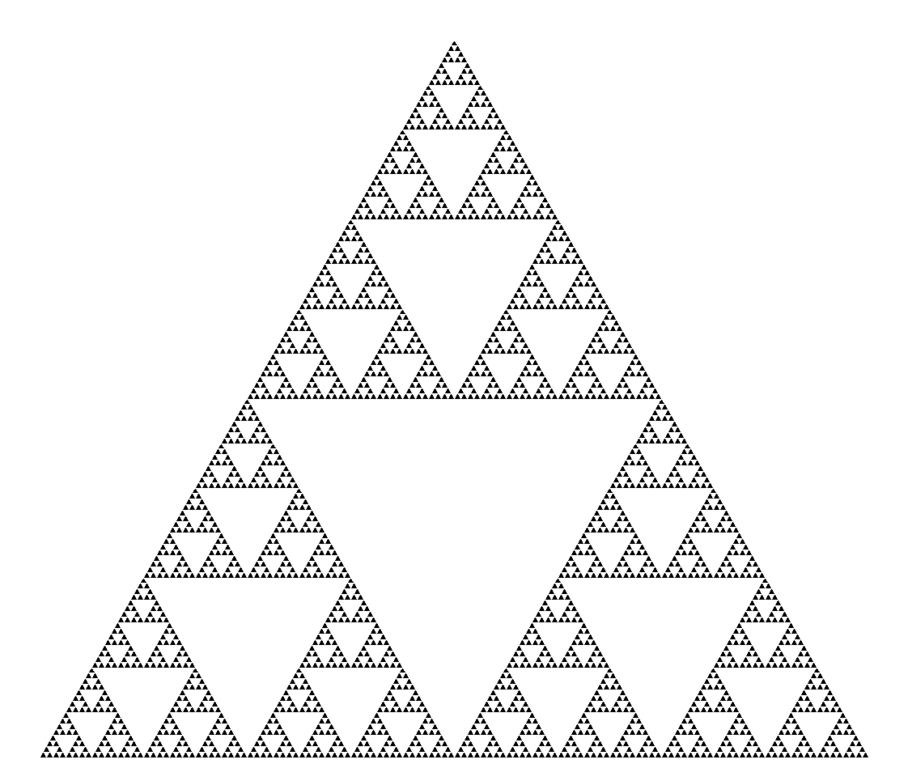
\includegraphics[scale=0.2]{sierpinski-triangle.png}}
        \begingroup
        \captionof{figure}{Trikotnik Sierpinskega kot primer samopodobnega fraktala. \emph{Vir: }\url{https://www.gresham.ac.uk/search?terms=Biographer}}
        \endgroup

        \addvspace{0.5cm}
        Zaradi tehnike grajenja fraktalov iz vedno manjših podenot lahko vidimo kako se v obliki pojavi samopodobnost, ampak za uporabo fraktalov v primerih resničnega življenja to ne zadošča.
        Samopodobnost se seveda nahaja v naravi, vendar ni pogosta.
        Benoit Mandelbrot, kot matematik 20. stoletja, ni bil zadovoljen z posploševanjem grobih oblik narave v preprostejše oblike kot krivulje.
        Bil je mnenja, da so fraktali lahko orodje s katerim natančneje opišemo naravo.
        V naravi oblike niso pravilne, saj se ob povečavi ta oblika ne posploši, vendar pa je groba na vseh ravneh.
        Ideja pojava grobosti na vseh povečavah oblike je skoraj enaka ideji fraktala, da je oblika prvotnega telesa vidna na vseh ravneh.
        V definicijo je bila vpeljala ideja fraktalne dimezije (o kateri je napisano več v naslednjem podpoglavju), ki nam omogoči, razširitev fraktalov na nenavadne oblike, ki ohranjajo grobost ali nepravilnost pri vseh povečavah.
        Mandelbrot je v svoji knjigi "The Fractal Geometry of Nature" fraktale definiral kot oblike, katerih "Hausdorffova dimenzija" (dimenzije katerih vrednost je lahko realno število) presega "topološko dimenzijo" (dimenzije celih vrednosti).
        Na žalost tudi ta definicija sama po sebi ni popolna, saj se pojavijo izjeme, ki imajo Hausendorffovo dimenzijo enako topološki dimenziji.
        \cite{FractalDefinitionVideo}
        \cite{HausdorffDimension}\\

        Z vsem tem je fraktal mogoče neformalno definirati kot množico, ki ima vsaj nekatere od naslednjih lastosti:
        \cite{irvsic2015fraktalna}
        \begin{itemize}
            \item je samopodobna
            \item njena dimenzija presega njeno topološko dimenzijo
            \item ima nepravilno obliko
            \item ni diferenciabilna (v primeru grafa funkcije)
            \item ohranja podrobnosti pri vsaki povečavi
            \item ima rekurzivno definicijo
        \end{itemize}

    \subsection{Fraktalna dimenzija}
        Za razumevanje fraktalne dimenzije, moramo najprej pogledati lastnosti celih dimenzij.
        Za začetek vzamemo za primer daljico, ki ima dimenzijo 1 in dolžino $d$.
        Če daljico presekamo na pol, dobimo dve novi daljici z dolžino $\frac{d}{2}$.
        
        \addvspace{0.5cm}
        \begin{tikzpicture}
            \draw[thick] (0,0) -- (4,0);
            \node at (2,-0.3) {$d$};
            \draw[thick] (6,0) -- (8,0);
            \draw[thick] (8.5,0) -- (10.5,0);
            \node at (7,-0.3) {$\frac{d}{2}$};
            \node at (9.5,-0.3) {$\frac{d}{2}$};
        \end{tikzpicture}

        \addvspace{0.3cm}
        To lahko storimo tudi z kvadratom, ki ima 2 dimenziji in dolžino stranice $d$.
        Če prvotnemu kvadratu zmanjšamo stranico na $\frac{d}{2}$, dobimo štriri nove kvadrate s četrtino ploščine.

        \addvspace{0.5cm}
        \begin{tikzpicture}
            \draw[thick] (0,0) rectangle (4,4);
            \node at (2,-0.3) {$d$};
            \draw[step=2cm,thick] (6,0) grid (10,4);
            \node at (7,-0.3) {$\frac{d}{2}$};
            \node at (9,-0.3) {$\frac{d}{2}$};
        \end{tikzpicture}

        \addvspace{0.3cm}
        Ta postopek lahko razširimo na višje dimenzije.
        V treh dimenzijah dobimo rezultat 8 novih kock s polovično dolžino stranice.
        V štirih dimenzijah dobimo 16 novih teseraktov s polovično dolžino stranice in tako naprej.\\
        
        Možno je tudi stranice skrčiti z dugačnimi faktorji.
        Za primer lahko vzamemo tretjine.
        V prvi dimenziji s črto tako dobimo 3 nove črte z tretjino dolžine.
        V drugi dimenziji s kvadratom dobimo 9 novih kvadratov s stranico dolgo tretjino originalne.
        V tretji dimenziji s kocko dobimo 27 novih kock s stranico dolgo tretjino originalne.
        To lahko nadaljujemo v višje dimenzije.\\
        
        Viden je vzorec, število manjših kopij se s povečanjem dimenzije za 1 poveča za obratno vrednost faktorja krčenja.
        Če to posplošimo v formulo, kjer je $N$ število kopij, $D$ dimenzija in $r$ faktor krčenja ($0<r<1$), dobimo naslednje:
        \[N=\left(\frac{1}{r}\right)^D\]
        V primeru, da kopijo poskušamo razširiti je $r$ faktor širjenja ($r>1$), pa dobimo naslednji izraz:
        \[N=r^D\]
        Ko izrazimo dimenzijo pa se nam pojavi naslednja formula:
        \[D=\frac{\log{N}}{\log{\left(\frac{1}{r}\right)}}\]\\
        Ali:
        \[D=\frac{\log{N}}{\log{r}}\]

        \addvspace{1cm}
        Običajne oblike, kot črte in kvadrate, lahko izmerimo z enodimenzionalnimi merami, dvodimenzionalnimi merami in tako naprej.
        Primer tega so metri, dolžino merimo v metrih, ploščino v kvadratnih metrih, volumen v kubičnih metrih in tako naprej.
        Te mere pa pri naših fraktalih ne zadostujejo.
        Na sliki spodaj je narisana Kochova krivulja, ki na prvi pogled izgleda kot navadna črta z začetno in končno točko, vendar je njena dolžina neskončna.
        Ni važno kako blizu pogledamo in probamo izmeriti dolžino krivulje, spet bomo naleteli na enako krivuljo kot na začetku.
        Prav tako je ploščina krivulje nič, saj je narejena zgolj iz črt, ki pa nimajo ploščine.
        Tako vemo, da se Kochova krivulja nahaja nekje med 1. in 2. dimenzijo, saj je z enodimenzionalnimi merami neskončno dolga, z dvodimenzionalnimi pa dobimo rezultat 0.
        Če bi hoteli izmeriti Kochovo krivuljo, bi potrebovali mere, ki zadostujejo njeni dimenziji.
        \cite{FractalDefinitionVideo}
        \cite{FractalDefinition}
        \centerline{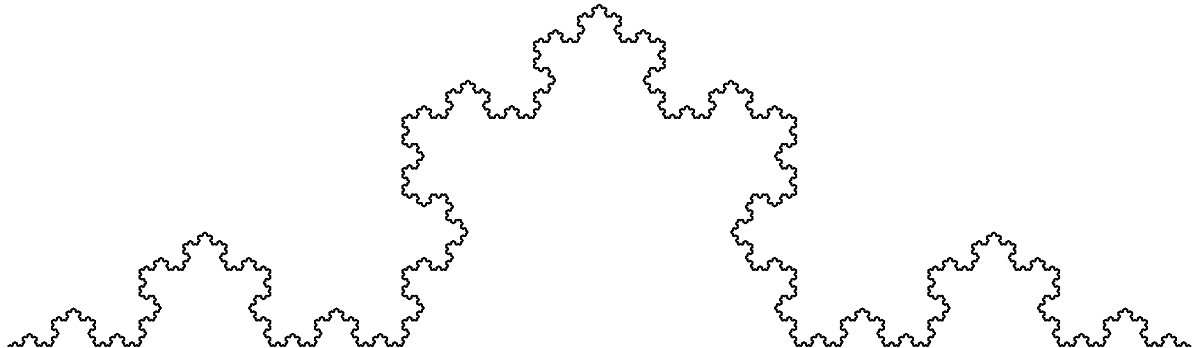
\includegraphics[scale=0.2]{koch-curve.png}}
        \begingroup
        \captionof{figure}{Kochova krivulja z neskončno dolžino in ploščino nič. \emph{Vir: }\url{https://\\youwei96.wixsite.com/messyworkings/single-post/2016/06/11/area-of-the-koch-curve}}
        \endgroup

        \addvspace{0.5cm}
        Da izračunamo dimenzijo fraktala pa lahko uporabimo formulo, ki smo jo odkrili prej.
        Za primer lahko vzamemo Kochovo snežinko, ki je narisana na zgornji sliki.
        Potrebujemo dva podatka, koeficient skrčenja $r$ in število kopij $N$.
        Ker je Kochova krivulja narejena tako, da črto razdelimo na tretjine in srednji del zamenjamo s trikotnikom brez spodnje stranice je primerno vzeti $r=\frac{1}{3}$.
        Če Kochovo krivuljo skrčimo, vidimo, da lahko originalno krivuljo zgradimo iz $N=4$ kopij nove krivulje.
        \cite{FractalDimensionsVideo}
        \centerline{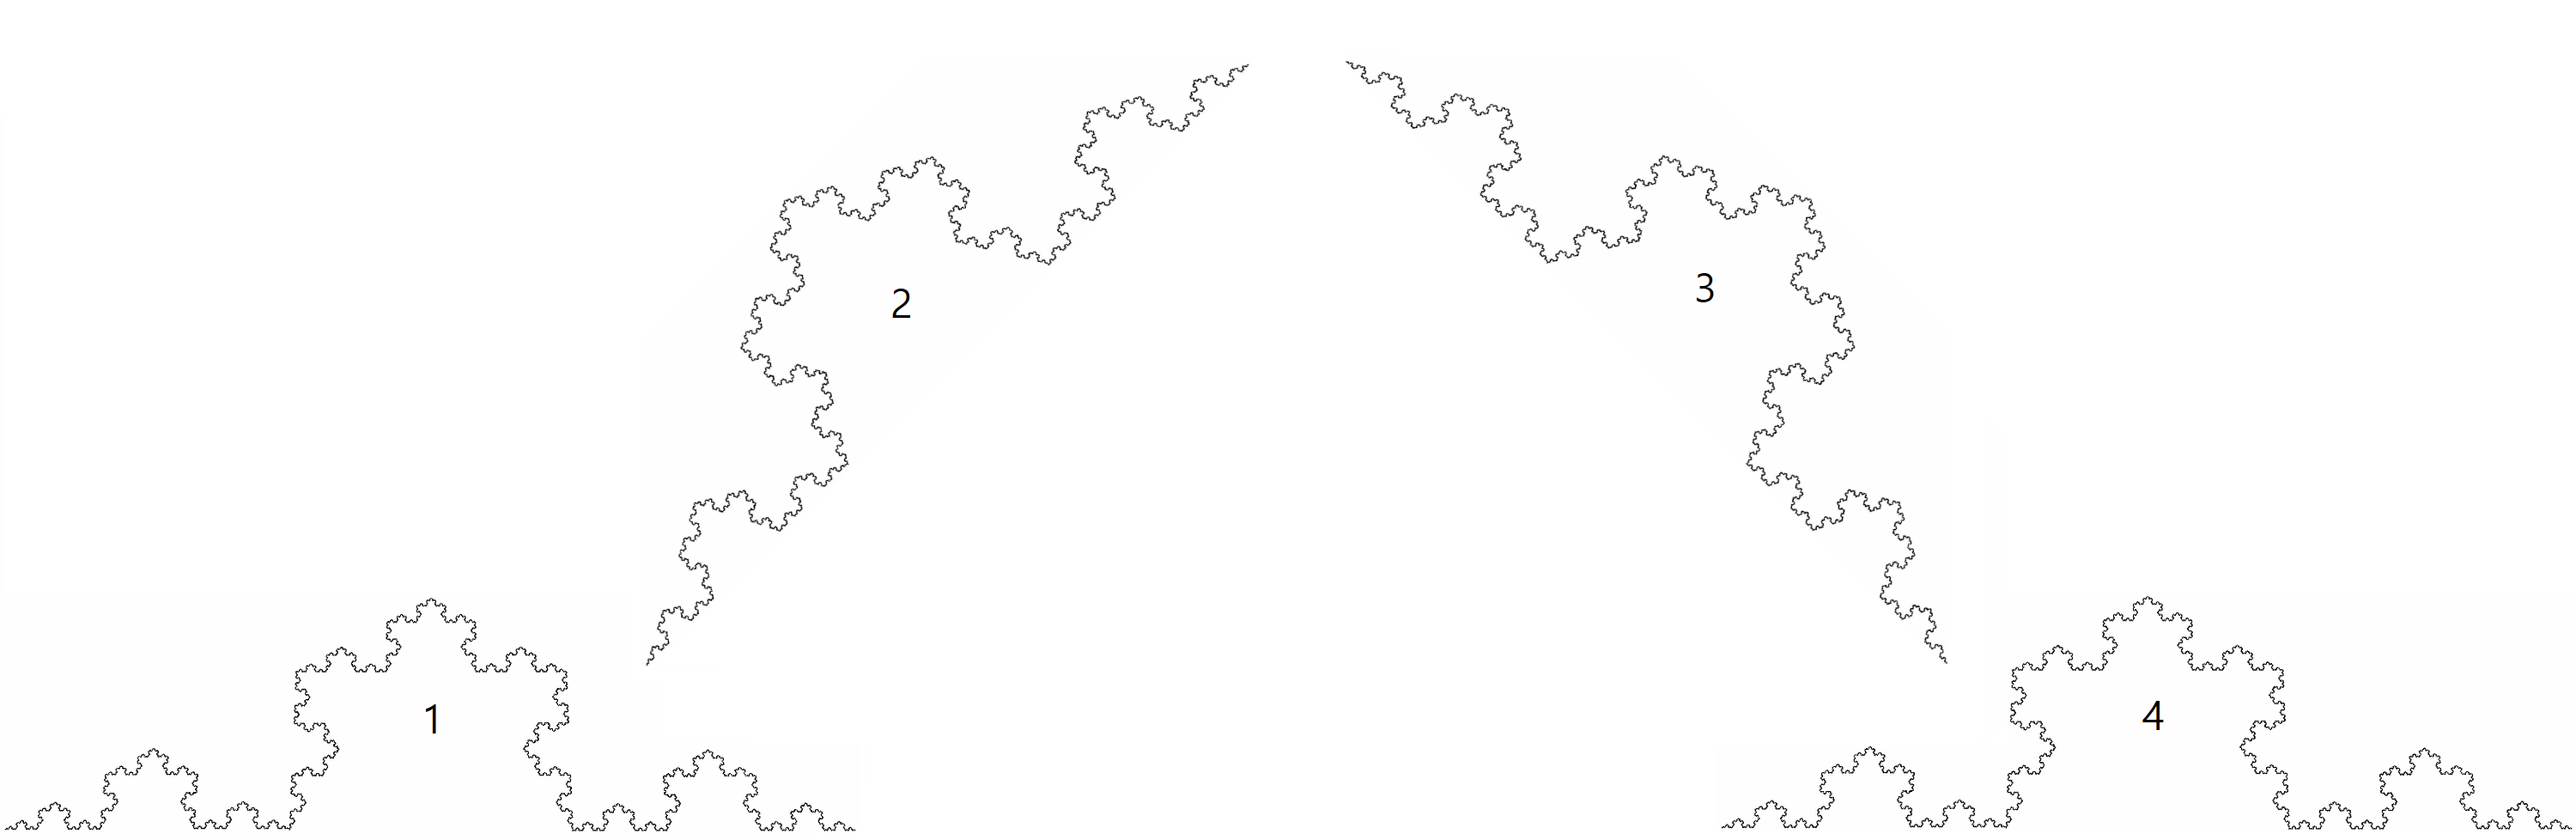
\includegraphics[scale=0.2]{koch-curve-dimension.png}}
        \begingroup
        \captionof{figure}{Kochova krivulja zgrajena iz štirih Kochovih krivulj z dolžino 1/3 originalne}
        \endgroup

        \addvspace{0.5cm}
        Če te podatke vstavimo v formulo in jo vnesemo v kalkulator, dobimo naslednje:
        \[D=\frac{\log{4}}{\log{3}}\approx1,26\]

\section{Risanje fraktalov}
    \subsection{Iterativni funkcijski sistem}
        Iterativni funkcijski sistem je eden od načinov prikazovanja fraktalov, pri čemer je končni rezultat po navadi samopodobni fraktal.
        Ideja za delovanjem sistema je sestavljenost frarktala iz mnogih enakih podenot na katerih je bila uporabljena določena funkcija.
        Večina teh funkcij je kontraktivnih, kar zmanjšuje razdalje med točkami in posledično tudi oblike.
        Od tod samopodobnostne lastnosti tega načina prikazovanja.
        \cite{IFS}\\

        Eden najzanimivejših primerov Iterativnega funkcijskega sistema je igra kaosa, kjer iz na pogled čisto naključne igre dobimo fraktalne oblike.
        Za risanje trikotnika Sierpinskega sledimo naslednjim navodilom.
        Kot osnovno obliko si izberemo trikotnik in v ravnino narišemo samo ogljišča tega trikotnika.
        Nato si v ravnini izbermo poljubno točko (lahko je znotraj ali zunaj trikotnika).
        Naključno izberemo eno od treh ogljišč in se premaknemo na polovico daljice, ki je nastala med poljubno točko in naključnim ogljiščem.
        Spet naključno izberemo eno od treh ogljišč, vendar se tokrat pomaknemo na polovico daljice med novonastalo točko in naključnim ogljiščem.
        To ponavljamo za vse novonastale točke in se nam po določenem času nariše trikotnik Sierpinskega, saj je možnost, da točka pristane v praznini trikotnika Sierpinskega enaka nič (razen če je bila tja postavljena prvotna točka).
        \cite{ChaosGame}\\

        Če podobno ponovimo na kvadratu, le da istega ogljišča ne smemo izbrati dvakrat zapored se nam pojavi naslednji fraktal:
        \centerline{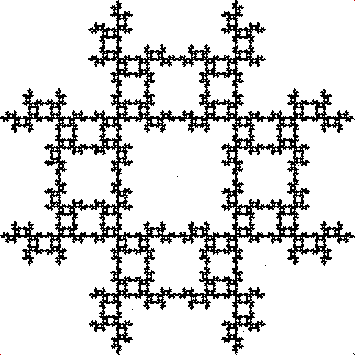
\includegraphics[scale=0.6]{square-fractal.PNG}}
        \begingroup
        \captionof{figure}{Igra kaosa na kvadratu. \emph{Vir: }\url{https://www.wikiwand.com/en/Chaos_game}}
        \endgroup
    
    \subsection{L-sistem}
        L-sistem ali Lindenmayerov sistem je vrsta gramatike, ki je zmožna zelo dobro definirati rekurzivne strukture.
        Sisteme je ustvaril Aristid Lindenmayer, biolog in botanist, ko je iskal način prikazovanja rasti celičnih organizmov in rastlin.
        Le kot dodatek je zaradi rekurzivne narave teh sistemov danes mogoče z njimi ustvariti tudi fraktale.
        L-sistemi za delovanje potrebujejo "abecedo" ali spremenljivke in konstante, aksiom ali začetni niz simbolov ter pravila, ki prehodnim nizom spremenljivk določijo nov niz elementov "abecede".
        Z iteracijo ustvarjamo izhodni niz, katerega pomen iterpretiramo kot navodila za risanje določene oblike.
        \cite{LSystem}\\

        Za primer lahko vzamemo sistem z spremenljivkama $A$ in $B$, aksiomom $A$ in pravili $A \rightarrow AB$ in $B \rightarrow A$. ($n$ predstavlja število iteracij):
        \begin{itemize}
            \item[] $n=0: A$
            \item[] $n=1: AB$
            \item[] $n=2: ABA$
            \item[] $n=3: ABAAB$
            \item[] $n=4: ABAABABA$
            \item[] $n=5: ABAABABAABAAB$
        \end{itemize}

        \addvspace{0.5cm}
        Za risanje fraktalov z L-sistemi definiramo eno spremenljivko ali več spremenljivk kot risanje črte v določeno smer z določeno dolžino.
        Poleg tega pa definiramo še konstante $+$, kar pomeni obrat v levo za določen kot, $-$, obrat v desno za določen kot, $[$, shrani trenuten položaj ter $]$, ki povrne sistem v nazadnje shranjen položaj.
        To nam omogoča risanje dvodimenzionalnih oblik ter risanje razvejanih oblik.
        Za primer imamo trikotnik Sierpinskega, kjer $F$ in $G$ oba pomenita risanje črte:
        \cite{LSystem}
        \begin{itemize}
            \item[] spremenljivke: $F, G$
            \item[] konstante: $+, -$
            \item[] aksiom: $F-G-G$
            \item[] kot obračanja: $120^\circ$
            \item[] pravila: $F \rightarrow F-G+F+G-F$ in $G \rightarrow GG$    
        \end{itemize} 

    \subsection{Končno delitveno pravilo}
        Končno delitveno pravilo je rekurzivni način deljenja večkotnikov in drugih dvodimenzionalnih oblik na manjše dele.
        To nam omogoča izdelovanje geometričnih fraktalov, vendar nam vseeno dopušča delne spremembe pri vsakem koraku.
        Končno delitveno pravilo razdeli določeno teselacijo ali tlakovanje (pokritje ravnine z geometriskimi liki) in jo spremeni v novo teselacijo iz manjših večkotnikov.
        Končno je zgolj takrat, ko je različnih načinov deljenja večkotnikov.
        En način deljenja večkotnika imenujemo vrsta ploščice in en način deljenja roba oblike vrsta roba.
        \cite{FSR}
        \centerline{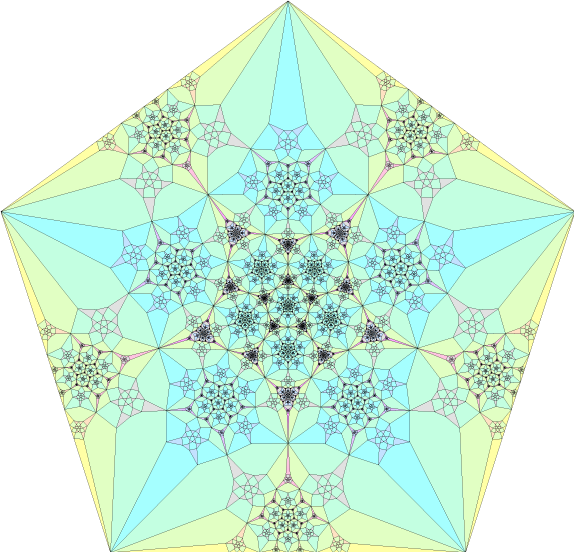
\includegraphics[scale=0.3]{fsr-fractal.png}}
        \begingroup
        \captionof{figure}{Fraktal narejen s končnim delitvenim pravilom. \emph{Vir: }\url{https://www.pinterest.com/pin/422353271298859809/}}
        \endgroup

    \subsection{Escape-time fraktali}
        To so fraktali narejeni z uporabo formule ali ponovitvene relacije (enačba, ki rekurzivno definira zaporedje kot elemente, katerih vrednost je enaka funkciji prejšnjega elementa).
        Z uporabo formule ali ponovitvene relacije na vsaki točki se nam lahko pojavijo fraktali.
        Najbolj poznan primer teh fraktalov je Mandelbrotova množica, ki je množica točk $c$ v kompleksni ravnini za katere neskončno zaporedje iteracije kompleksnega polinoma $z_n=z_{n-1}+c$ je omejeno.
        Pod to skupino spadajo še naslednji fraktali: Julijeva množica, Lyapunov fraktal, fraktal goreče ladje in še mnogo drugih.
        \cite{FractalDefinition}
        \cite{MandelbrotSet}
        \centerline{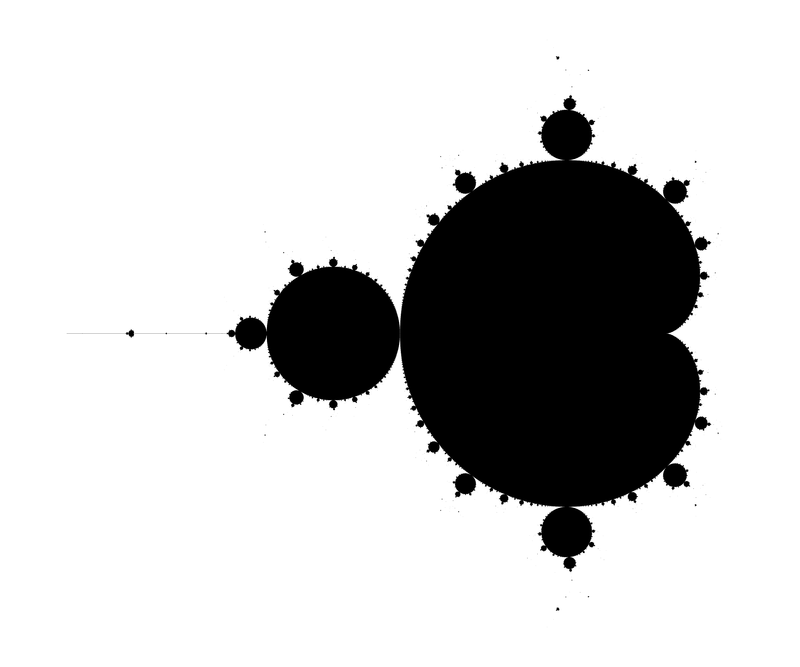
\includegraphics[scale=1.2]{mandelbrot-set.png}}
        \begingroup
        \captionof{figure}{Mandelbrotova množica. \emph{Vir: }\url{https://www.math.univ-toulouse.fr/~cheritat/wiki-draw/index.php/Mandelbrot_set}}
        \endgroup

\listoffigures
\printbibliography

\end{document}